\section{Cilindro}


\begin{frame}[fragile]{Definição}

    \begin{itemize}
        \item O cilindro é uma figura geométrica formada pelos pontos equidistantes de 
            um eixo (segmento de reta) dado
        \pause

        \item Esta distância fixa recebe o nome de raio $r$
        \pause

        \item Em geral, um cilindro é representado pelo raio e pela distância entre as 
            duas faces circulares opostas, denominada altura $h$
        \pause

    \end{itemize}

    \begin{figure}
        \centering
        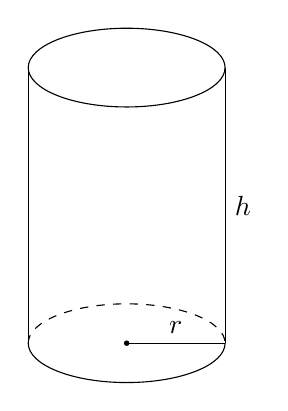
\begin{tikzpicture} %[>=latex,shorten >=2pt,shorten <=2pt,shape aspect=1]
            \draw (0,0) ellipse (1.25 and 0.5);
            \draw (-1.25,0) -- (-1.25,-3.5);
            \draw (-1.25,-3.5) arc (180:360:1.25 and 0.5);
            \draw [dashed] (-1.25,-3.5) arc (180:360:1.25 and -0.5);
            \draw (1.25,-3.5) -- node[anchor=west] { $h$ } (1.25,0);  
            \draw (0, -3.5) -- node[anchor=south] { $r$ } (1.25, -3.5);
            \fill (0, -3.5) circle [radius=1pt];
        \end{tikzpicture}
    \end{figure}
\end{frame}

\begin{frame}[fragile]{Área e volume}

    \begin{itemize}
        \item A área do cilindro é dada por 
        \[
            A = 2\pi rh + 2\pi r^2 = 2\pi r(h + r),
        \]
        isto é, sua área lateral (um retângulo de base $2\pi r$, que é a circunferência
            do círculo, e altura $h$) e o dobro da área da base ($\pi r^2$)
        \pause

        \item O volume, por sua vez, pode ser computado de duas formas
        \pause

        \item Uma delas é a integral de área usando coordenadas cilíndricas 
        \begin{align*}
            x &= r\cos \theta\\
            y &= r\sin \theta\\
            z &= z,
        \end{align*}
        onde $0 \leq \theta \leq 2\pi$
        \pause

        \item Outra é calcular a superfície de revolução de um segmento vertical de comprimento
            $h$ no ponto $x = r$ torno do eixo $y$
        \pause

        \item Em ambos casos, $V = \pi r^2 h$, que é igual a área da base vezes a altura

    \end{itemize}

\end{frame}

\begin{frame}[fragile]{Implementação de um cilindro}
    \inputcode{cpp}{codes/cylinder.cpp}
\end{frame}
